\documentclass[12pt]{article}

\usepackage{a4wide} % уменьшает поля
\usepackage[utf8]{inputenc}
\usepackage[russian]{babel} % включает русский язык
\usepackage{graphicx} % позволяет подключить .eps - файлы
\usepackage{amsmath}
\usepackage{amsthm} % теоремы от AMS
\usepackage{amssymb} % для работы с математическими R и проч.
\usepackage{floatrow}
\usepackage{mathrsfs}
\usepackage[section]{placeins}
\usepackage{indentfirst} % абзац после заголовка
\usepackage{misccorr} % точки в заголовках

%\graphicspath{{pics/}}


%\newtheoremstyle{rusdef}
%  {3pt}% measure of space to leave above the theorem. E.g.: 3pt
%  {3pt}% measure of space to leave below the theorem. E.g.: 3pt
%  {\itshape}% name of font to use in the body of the theorem
%  {\parindent}% measure of space to indent
%  {\bfseries}% name of head font
%  {.}%
%  {.5em}%
%  {}
   
  
\theoremstyle{rusdef}
\renewcommand\qedsymbol{$\blacksquare$}
\newtheorem{remark}{Замечание}
\newtheorem{theorem}{Теорема}
\newtheorem{definition}{Определение}
\newtheorem{proposition}{Утверждение}

\newcommand*{\hm}[1]{#1\nobreak\discretionary{}{\hbox{$\mathsurround=0pt #1$}}{}}
\newcommand{\scalar}[2]{\left<#1,#2\right>}
\newcommand{\const}{\ensuremath{\operatorname{const}}}
\newcommand{\sgn}{\ensuremath{\operatorname{sgn}}}
\renewcommand{\d}[1]{\ensuremath{\operatorname{d}\!{#1}}}
\newcommand\abs[1]{\left\lvert #1 \right\rvert} % модуль
\newcommand\brackets[1]{\left( #1 \right)} % скобки
\newcommand{\R}{\ensuremath{\mathbb{R}}} % R - мн-во вещественных чисел
\newcommand{\N}{\ensuremath{\mathbb{N}}} % N - мн-во натуральных чисел
\newcommand{\Z}{\ensuremath{\mathbb{Z}}} % Z - мн-во целых чисел
\renewcommand{\C}{\ensuremath{\mathbb{C}}} % C - мн-во комплексных чисел
\newcommand{\E}{\ensuremath{\mathcal{E}}} % E --- эллипсоид
\newcommand{\norm}[1]{\left\lVert #1 \right\rVert} % норма
\DeclareMathOperator*{\thus}{\Rightarrow} % следствие с возможностью использовать limits
\DeclareMathOperator*{\tolim}{\to} % стремление с возможностью использовать limits
\DeclareMathOperator*{\Argmax}{Argmax} % Argmax с возмножностью использовать limits
\DeclareMathOperator{\rank}{rank} % ранг
\DeclareMathOperator{\e}{e} % экспонента

\newcommand{\rpm}{\sbox0{$1$}\sbox2{$\scriptstyle\pm$}
\raise\dimexpr(\ht1)/2\relax\box2 } % крутой плюс-минус

\begin{document}
\thispagestyle{empty}

\begin{center}
\ \vspace{-3cm}


\includegraphics[width=0.5\textwidth]{msu.eps}\\

{\scshape Московский Государственный Университет имени М.~В.~Ломоносова}\\
Факультет Вычислительной Математики и Кибернетики\\
Кафедра Системного Анализа
\vfill

{\LARGE Лабораторная работа по курсу <<Математические модели в экономике>>}

{\LARGE Анализ структуры потребительского спроса с помощью обобщённого непараметрического метода}
\vspace{.5cm}

\end{center}

\vspace{1cm}

\begin{flushright}
\large
\textit{Студент 415 группы}\\
В.~С.~Терёшин\\
\vspace{5mm}
\textit{Руководитель практики}\\
к.ф.-м.н., ассистент А.В.Рудева

\end{flushright}

\vfill

\begin{center}
{\large
Москва, 2014г.}
\end{center}

\newpage
\tableofcontents
\newpage
\section{Постановка задачи}
Найти три интегрируемые группы, построить графики экономических индексов для интегрируемой группы и для двух товаров из этой группы, построить индексы Ласпейреса и Пааше, сравнить. Сделать вывод об использовании индекса, построенного непараметрическим методом.
\section{Поиск интегрируемых групп}
Задание выполнялось по данным торговой статистики Венгрии за период 1975-1984 гг. Интегрируемые группы искались с помощью системы ИНДЕКС. Для этого перебирались несколько значений $\omega$ --- коэффициент отклонения потребителей от рационального поведения. В качестве параметра $\omega$ были взяты следующие значения: $0, 0.00005, 0.001, 0.01$. Оказалось, что с увеличением значения параметра $\omega$ число интегрируемых групп растёт. При $\omega = 0$ всего 2 интегрируемые группы, а при $\omega = 0.01$ уже 11 групп. Выделим 3 интегрируемые группы, т.е. остановимся на $\omega = 0.00005$ и получим, что интегрируемыми группами являются продовольственные товары, напитки и табачные изделия.
\begin{figure}[h!]
	\centering
	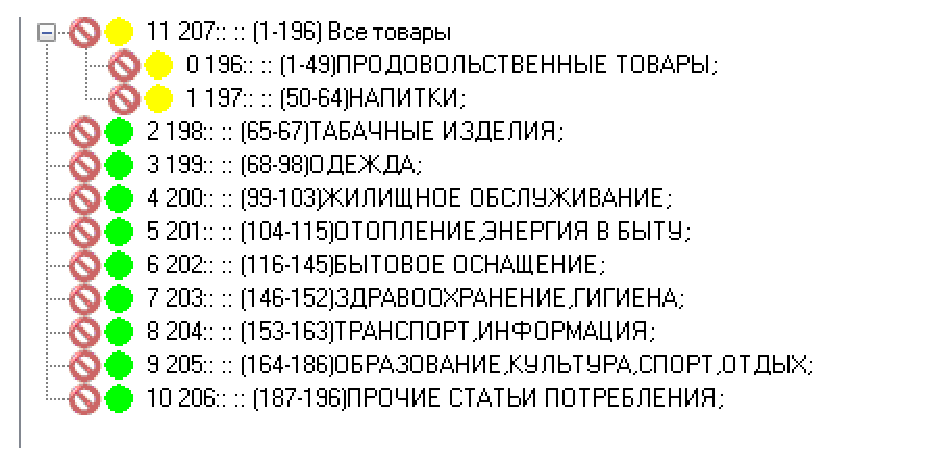
\includegraphics[scale=0.8]{pics/w0.eps}
	\caption{$\omega = 0$.}
\end{figure}
\begin{figure}[h!]
	\centering
	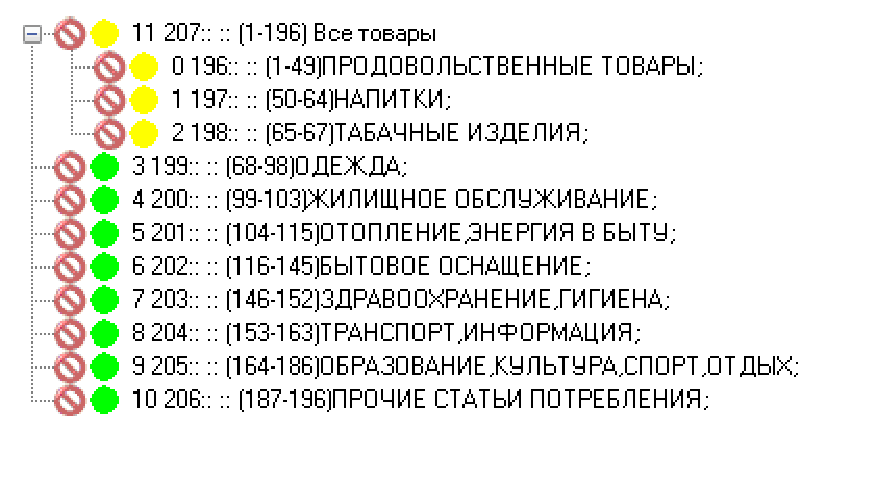
\includegraphics[scale=0.8]{pics/w0.00005.eps}
	\caption{$\omega = 0.00005$.}
\end{figure}
\begin{figure}[h!]
	\centering
	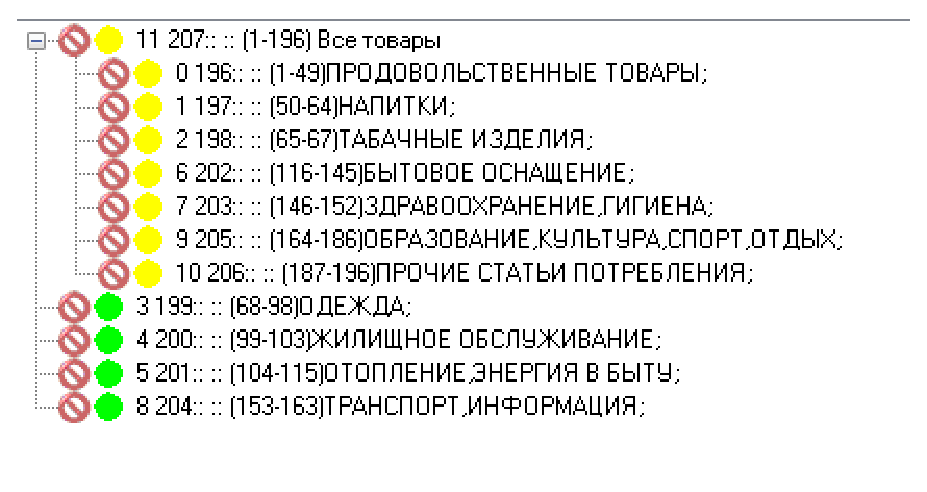
\includegraphics[scale=0.8]{pics/w0.001.eps}
	\caption{$\omega = 0.001$.}
\end{figure}
\begin{figure}[h!]
	\centering
	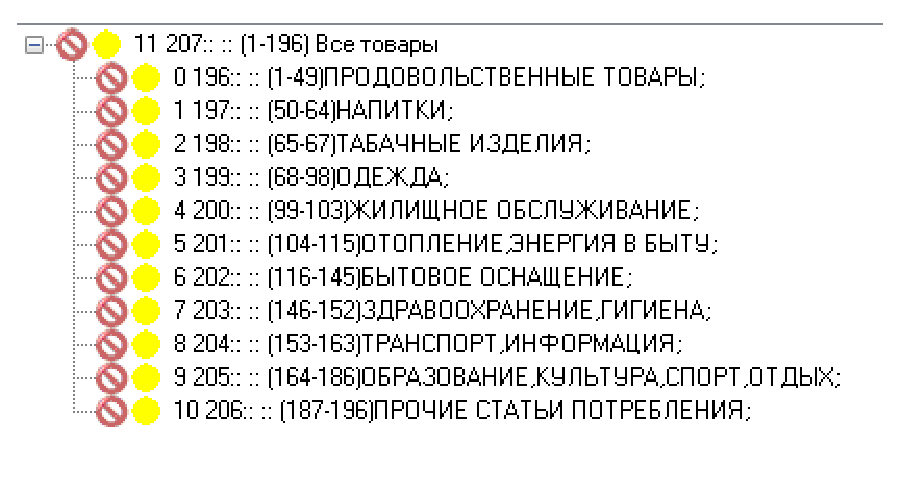
\includegraphics[scale=0.8]{pics/w0.01.eps}
	\caption{$\omega = 0.01$.}
\end{figure}
\section{Графики индексов интегрируемой группы и двух товаров из этой группы}
В качестве интегрируемой группы была взята группа <<Напитки>>. В качестве товаров были выбраны <<Кофе>> и <<Ром, водка>>.
\begin{figure}[h!]
	\centering
	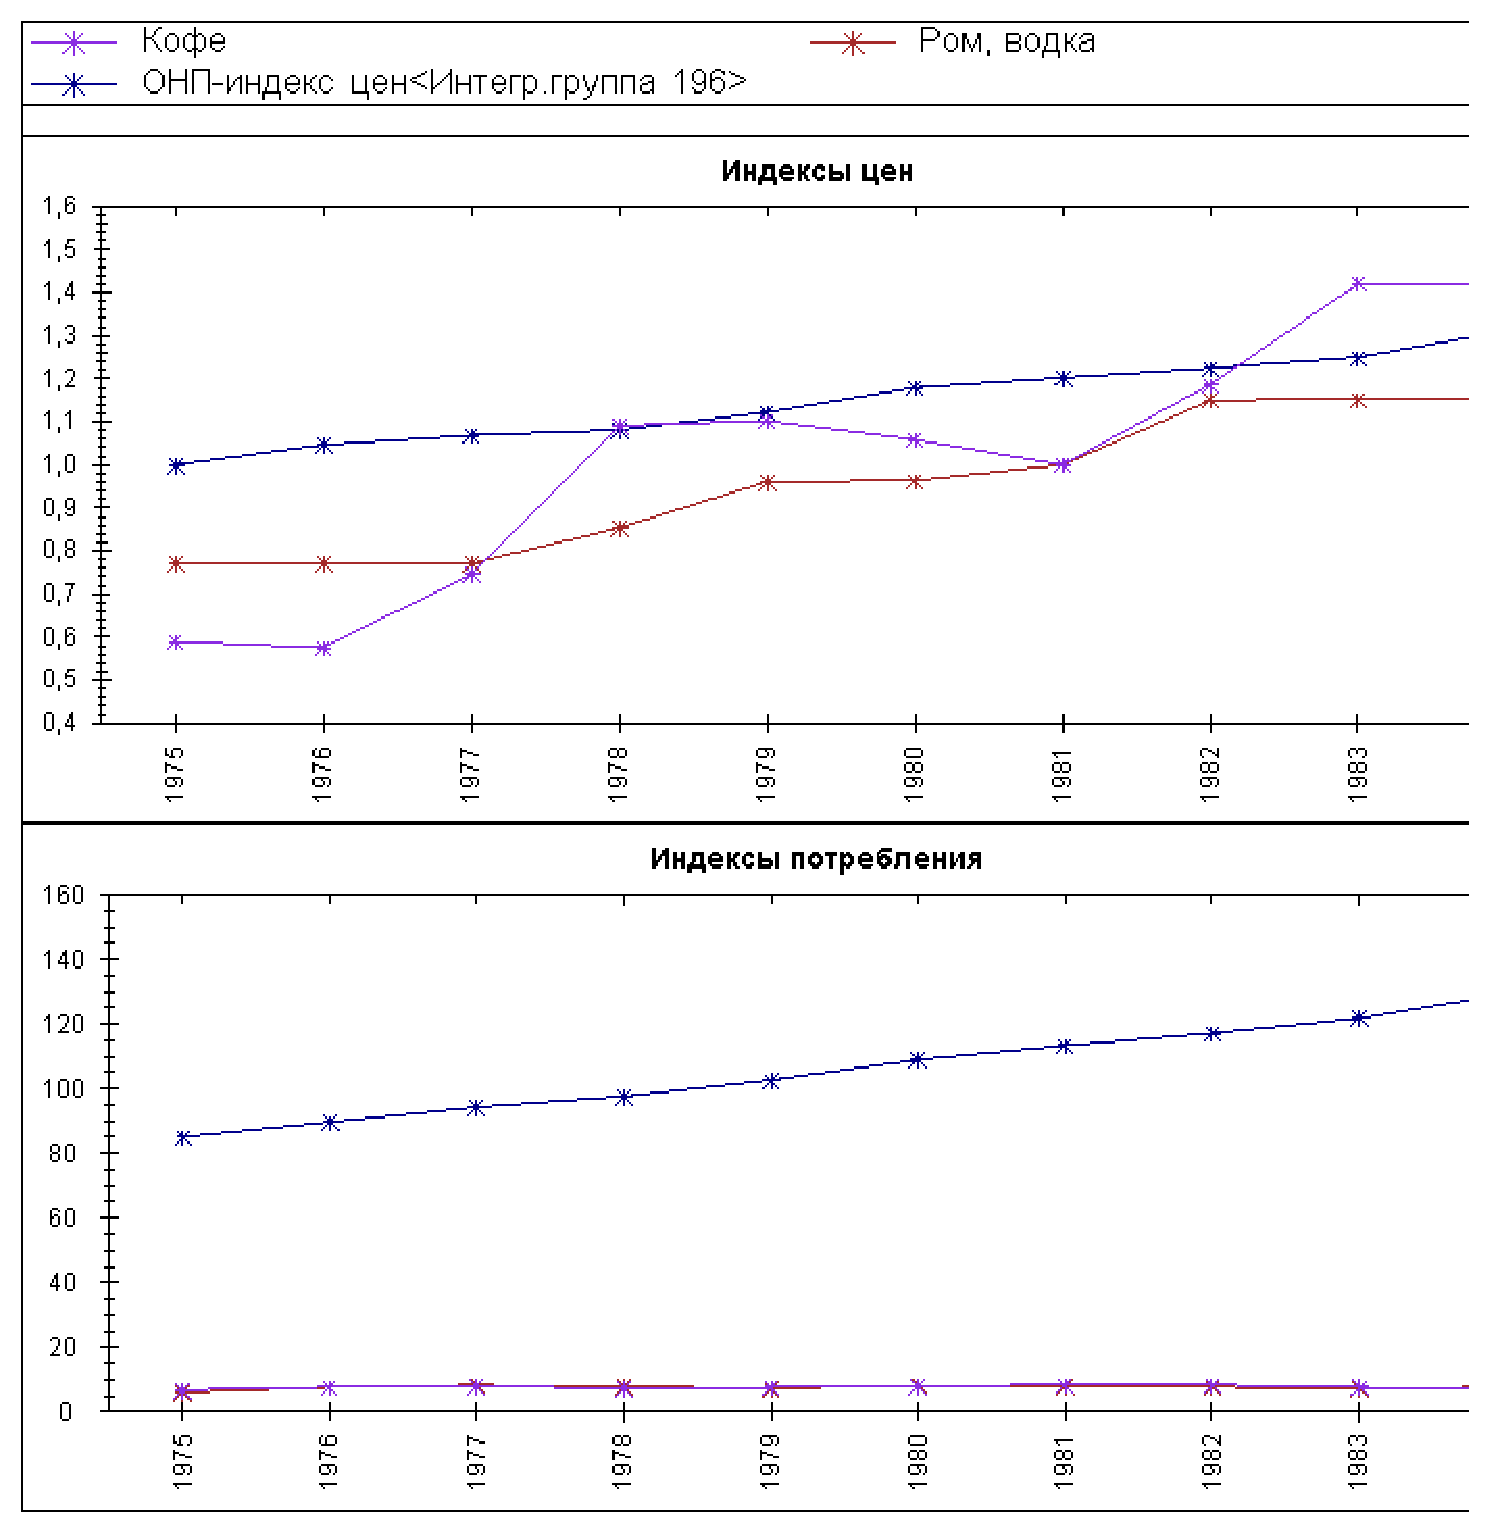
\includegraphics[scale=0.6]{pics/pic1.eps}
	\caption{}
\end{figure}
\section{Индекс Ласпейреса и Пааше}
В данном разделе индексы построены для двух групп: <<Продовольственные товары>> <<Напитки>>.
\begin{figure}[h!]
	\centering
	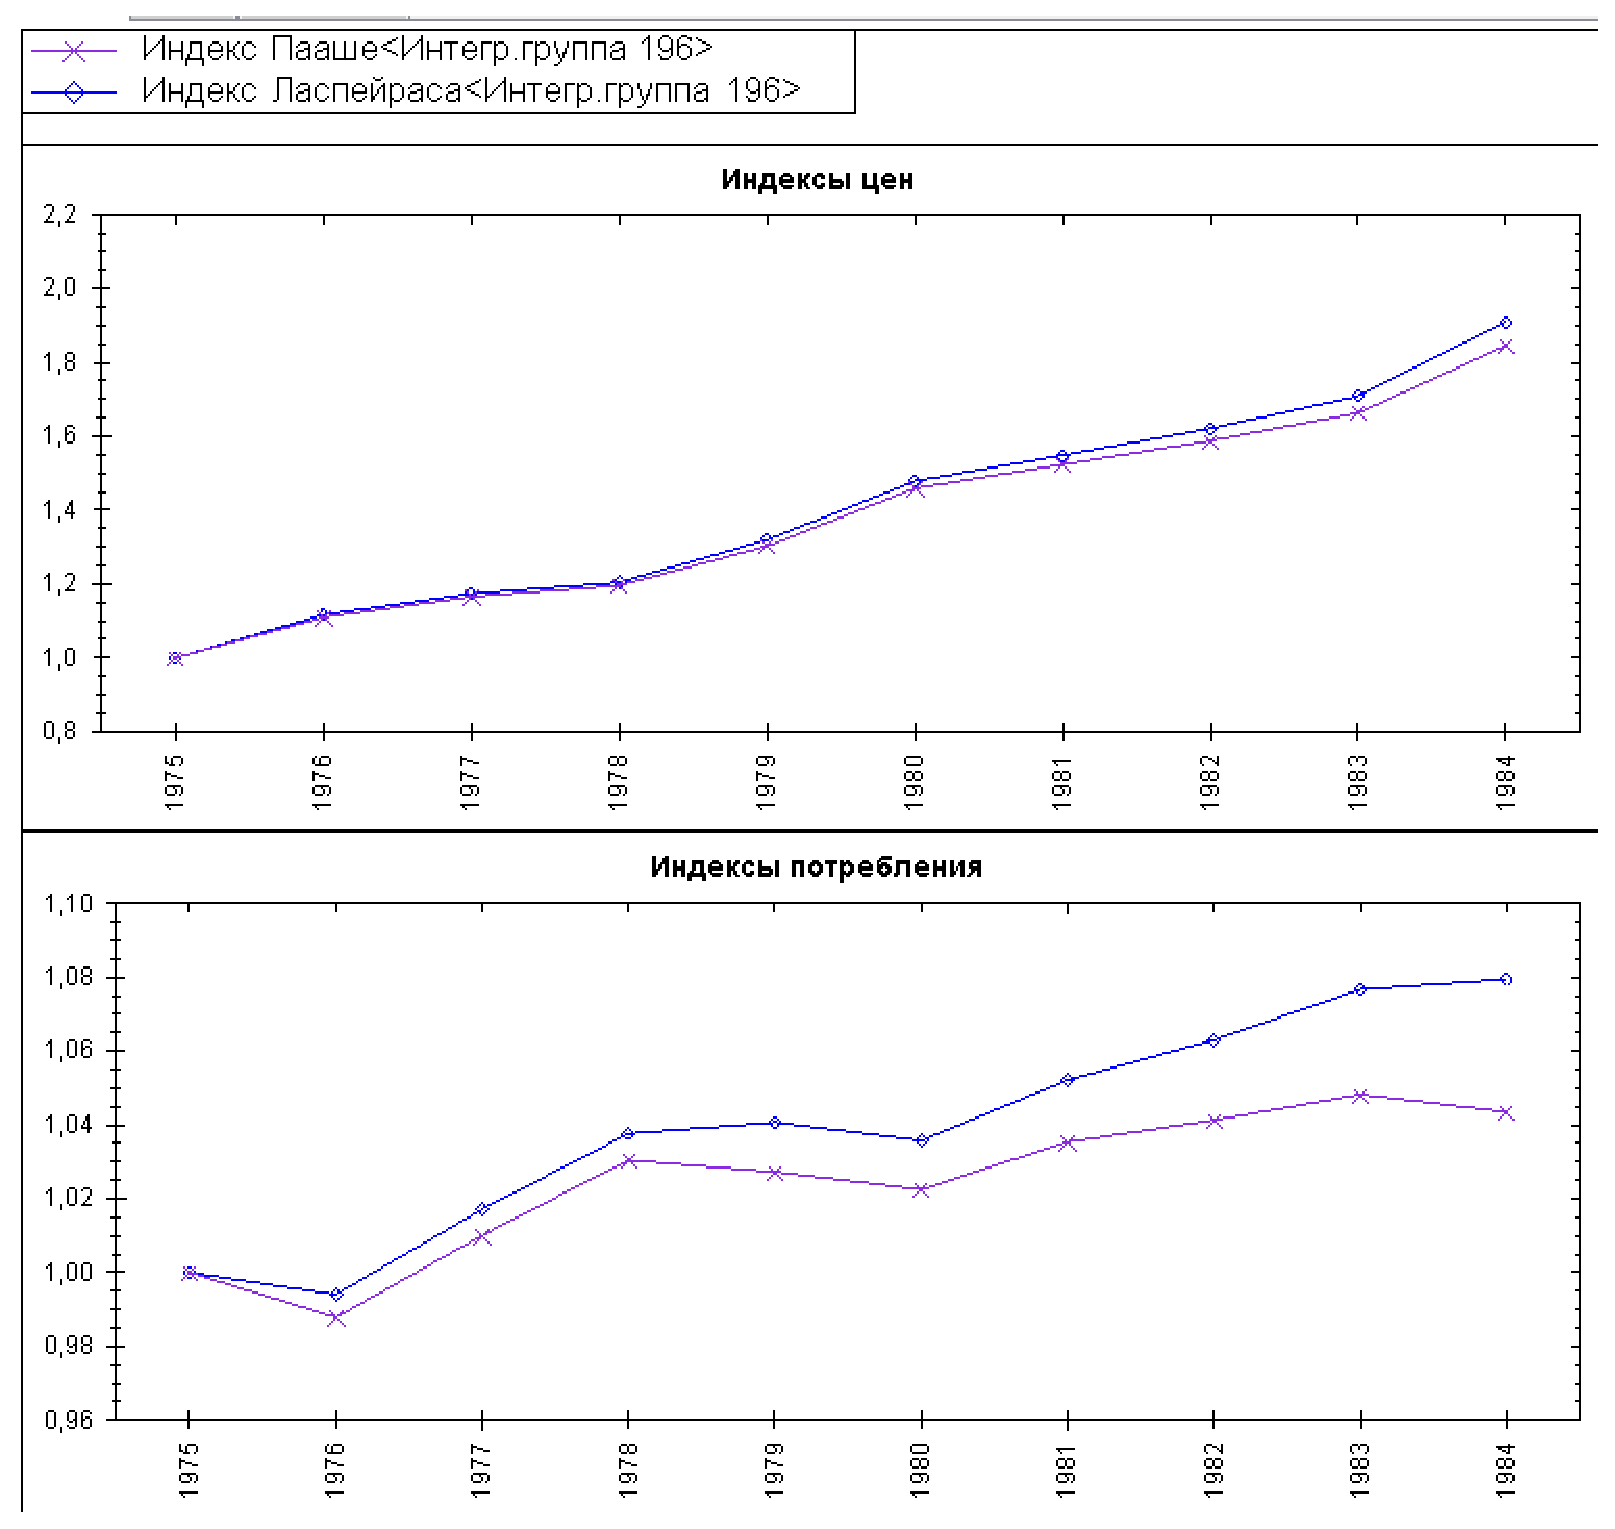
\includegraphics[scale=0.6]{pics/pic2.eps}
	\caption{Продовольственные товары}
\end{figure}
\begin{figure}[h!]
	\centering
	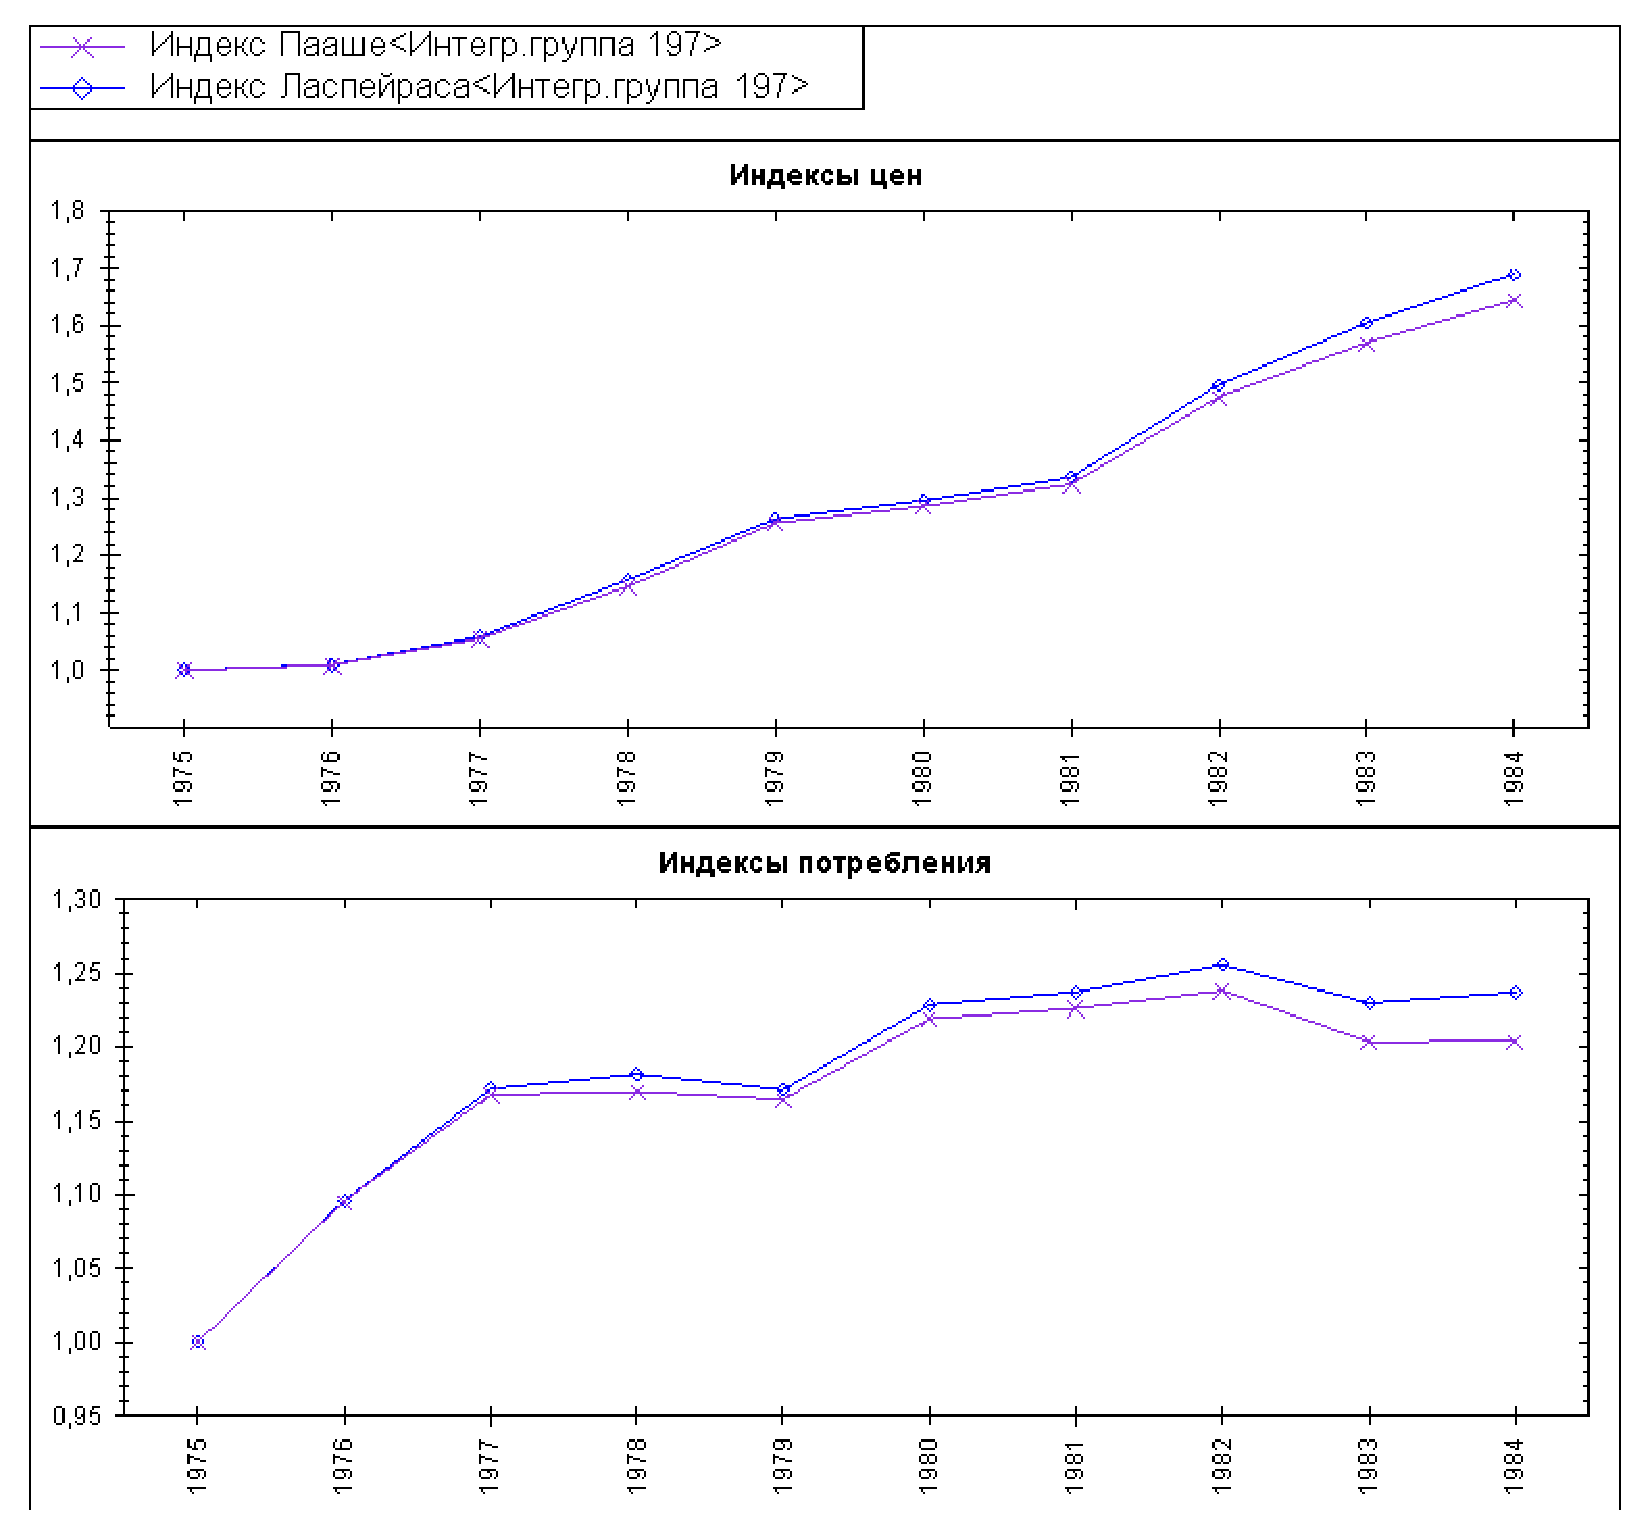
\includegraphics[scale=0.6]{pics/pic3.eps}
	\caption{Напитки}
\end{figure}

Индекс Ласпейреса предполагает взвешивание цен двух периодов по объёмам потребления товаров в базисном, а индекс Пааше --- по объёмам их потребления в текущем периоде. Однако, ни тот, ни другой индекс не дают верного представления об изменении цен, поскольку они не учитывают влияние этого изменения на структуру потребления. Очевидно, что если цена товара X возрастает, то покупки его снижаются и наоборот. Поэтому значение индекса Ласпейреса даёт преувеличенное представление об изменении цен в случае из роста, но преуменьшенное в случае их снижения. Наоборот, значение индекста Пааше даёт преумешенное представление об изменении уровня цен в случае их роста и преувеличенное в случае их снижения. И в любом случае индекс Ласпейреса оказывается выше индекса Пааше. В отличие от методов вычисления индексов Ласпейреса или Пааше непараметрический метод позволяет на основе проверки отделимости изучать сегментированность рынков.
%\newpage
%\begin{thebibliography}{99}
%        \bibitem{example} Example.
%\end{thebibliography}
\end{document}